\chapter{Serverless design patterns} \label{cha:patterns}

In this chapter we take a look at serverless design patterns. Design patterns describe commonly accepted, reusable solutions to recurring problems \parencite{hohpe2004enterprise}. A design pattern is not a one-size-fits-all solution directly translatable into software code, but rather a formalized best practice that presents a common problem in its context along a general arrangement of elements that solves it \parencite{gamma94designPatterns}. The patterns in this chapter are sourced from scientific literature on serverless computing as well as cloud provider documentation. Literature on object-oriented patterns \parencite{gamma94designPatterns}, SOA patterns \parencite{rotem12soa} and enterprise integration patterns \parencite{hohpe2004enterprise} was also reviewed for applicable practices.

Enterprise integration patterns, as serverless is all about integrations. \textcite{hohpe2004enterprise} present a number of asynchronous messaging architectures in the seminal book on EIP. While predating the whole serverless phenomenon the patterns are still relevant. Hohpe even demonstrated implementing one of his patterns on top of Google's serverless platform \href{http://www.enterpriseintegrationpatterns.com/ramblings/google_cloud_functions.html}{in a blog post}. E.g. patterns like Idempotent Receiver, Dead-letter Channel as well as the 4 more general integration styles of File Transfer, Shared Database, RPC and Messaging. Many patterns implemented internally by FaaS platforms already!

SOA patterns: FaaS functions are self-contained nanoservices these might have some relevance. SOA patterns \parencite{rotem12soa} include Saga, Decoupled Invocation and others. As with EIP, some patterns are already implemented by the FaaS platform.

FaaSification: \textcite{spillner17transformpython} describes an automated approach to transform monolithic Python code into modular FaaS units by partially automated decomposition. Doesn't really seem suitable for the web application migration process covered in this thesis but worth mentioning.

\section{Orchestration patterns} \label{sec:orchestrationPatterns}

The following patterns concern serverless function orchestration, i.e. managing control flow to compose functions together into more extensive workflows. The patterns here constitute synchronous, sequential workflows, whereas asynchronous workflows are described in section \ref{sec:eventPatterns}.

\subsection{Routing Function} \label{subsec:routingFunction}

\textbf{Problem:} How do we branch out execution flow based on request payload?

\begin{figure}[h]
  \centering
  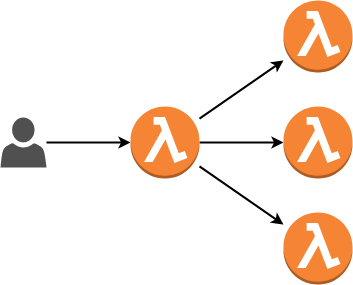
\includegraphics[width=0.5\textwidth]{patterns/routing-function.png}
  \caption{Routing Function}
  \label{fig:patternRoutingFunction}
\end{figure}

\textbf{Solution:} Use a central routing function to receive requests and forward them onwards to appropriate functions based on request payload.

This pattern involves instantiating a routing function that contains all the necessary information to route requests to other functions. All function invocations are directed to the routing function, which in turn dispatches requests onwards according to request payload.

It's notable that FaaS platforms commonly provide API gateways and other tools for routing, for example Amazon API Gateway \parencite{awslambda0218}. These tools are however mostly limited to path-based routing, whereas a routing function can be implemented to support more dynamic use cases. Also interestingly, according to an industry survey \parencite{leitner18industrialpractice}, some practicioners opted for the Routing Function pattern over platform API gateway services as they found the latter cumbersome to manage. One advantage of the pattern is that the routing function can be used to supplement request payload with additional context or metadata. A centralized routing function also means that all routing configuration is found in one place, and that public-facing API routes only need to be configured for one function, not all of them \parencite{leitner18industrialpractice}.

The pattern's major disadvantage is double billing, as the routing function essentially has to block and wait until the target function finishes execution. Strong coupling between the routing and target functions is another concern. Finally, as routing is implemented in function code level, routing information gets hidden in implementation rather than being accessible from configuration \parencite{leitner18industrialpractice}.

The Routing Function pattern is related to the OOP Command pattern, which aims to decouple clients from receivers via an intermediary command object \parencite{gamma94designPatterns}. A related enterprise integration pattern is Content-Based Router, which ``examines the message content and routes the message onto a different channel based on data contained in the message'' \parencite{hohpe2004enterprise}. \textcite{hohpe2004enterprise} caution that the router should be made easy to maintain as it can become a point of frequent configuration.

\subsection{Function Chain} \label{subsec:functionChain}

Chain functions to avoid timeouts.

\subsection{State Machine} \label{subsec:stateMachine}

AWS Step Functions etc. Caveat that (at least in AWS) step functions cannot be synchronously executed and are thus not composable functions themselves, i.e. a state machine cannot contain a state machine \parencite{lopez18orchestration}; \textcite{daly18blogPatterns} wraps step function in a function for this reason.
A more recent FaaS platform feature is function workflow or graph that enables composing functions together into more complex sequences akin to a state machine.

\subsection{Fat Client} \label{subsec:fatClient}

Let client orchestrate workflows.

\section{Event patterns} \label{sec:eventPatterns}

Asynchronous messaging/event patterns.

\subsection{Event processing} \label{subsec:Eventprocessing}

Trigger a function as a result of event occurrence.

\subsection{Periodic invocation} \label{subsec:periodicInvocation}

Schedule function invocations using cron-like systems.

\subsection{Fan-out events} \label{subsec:FanoutEvents}

Trigger multiple actions from a single event.

\subsection{Fan-out/fan-in} \label{subsec:FanoutFanin}

Split event handling into parallel functions.

\subsection{Pipes and filters} \label{subsec:PipesAndFilters}

Handle event stream with a pipeline of small functions.

\section{API/Integration patterns} \label{sec:apiPatterns}

Integrating with external systems.

\subsection{API composition} \label{subsec:apiComposition}

Hide multiple API calls under a single function.

\subsection{API aggregation} \label{subsec:apiAggregation}

Hide a sequential multi-step API call under a single function.

\subsection{API async} \label{subsec:apiAsync}

Turn a synchronized API into an async one.

\subsection{Legacy API Proxy/Staged migration} \label{subsec:legacyApi}

Replace a legacy API with a new one step by step, a.k.a. Strangler.

\subsection{Separate FaaS handler from core logic} \label
{subsec:separateHandler}

Separate FaaS handler core logic in code level.

\section{Data management/access patterns} \label{sec:dataManagementPatterns}

Managing state and accessing external resources.

\subsection{Externalized State} \label{subsec:externalizedState}

Store function state in external storage.

\subsection{Valet Key} \label{subsec:valetKey}

Sign tokens for clients to directly access resources.

\subsection{Least privilege IAM role} \label{subsec:LeastprivilegeIAMrole}

Minimize attack surface by reducing function access roles to bare minimum.

\section{Performance and scalability patterns} \label{sec:perfPatterns}

Address FaaS performance issues.

\subsection{Function warming} \label{subsec:FunctionWarming}

Ping a function intermittently to avoid cold starts.

\subsection{Oversized function} \label{subsec:OversizedFunction}

Choose maximum memory allocation to access faster CPU resources and improve cold start latency.

\subsection{Singleton} \label{subsec:Singleton}

Take advantage of function execution context to avoid reinitializing function dependencies.

\section{Resiliency and availability patterns} \label{sec:resiliencyPatterns}

Maximize serverless system resiliency.

\subsection{Bulkhead} \label{subsec:Bulkhead}

Isolate high-latency code into separate functions to avoid resource contention.

\subsection{Flow control/throttling} \label{subsec:Flow control/throttling}

Throttle invocations to avoid DDoSing yourself.

\subsection{Circuit breaker} \label{subsec:Circuit breaker}

Keep track of component availability to avoid cascading failures.

